\documentclass[11pt, letterpaper, onecolumn, oneside, final]{article}


\usepackage{lab}
\usepackage{soul}

\newfontfamily{\consolas}{Consolas}[Extension = .ttf]

\DocumentTitle {Project 0}
\DocumentSubtitle {Turtles!}
% End of preamble

%%%%%%%%%%%%%%%%%%%%%%%%%%%%%%%%%%%%%%%%%%%%%%%%%%%%%%%%%%%%%%%%%%%%%%%

\begin{document}
    \maketitle

    %\duedate{Weekday assigned: 0-6}{Week assigned: 0}{Weekday due:0-6}{Week due: 1}{Time due: 10:00 p.m.}
    \duedate{4}{0}{0}{3}{10:00 p.m.}

    \section{Collaboration.} Reminder of the collaboration policy: you may discuss the ideas of the project, but cannot share code or look at another student’s code. If you discuss, cite. More details are in the course syllabus.

    \section{Introduction.} In this project, you will be exploring the turtle module in Python and the sequential and iterative execution of code to create interesting images and designs. 
     
    \section{What to do.} Begin by downloading the {\consolas turtles.py} file from the class Piazza page. You can find it on the Resources page under Projects. Place it in a Project0 folder in the Projects folder in your CS101 directory. You can then open {\consolas turtles.py} in Thonny and begin the project. Be sure to save regularly, in case of any mishaps. Make sure to pay attention to the comments already in the file. \\
    \\
    Your task is to create an image, pattern, or graphic using turtles. You should draw upon your knowledge of turtles from Lab 1 and lectures. If you wish, you may also look into more advanced turtle techniques on your own, but if you do, be sure to cite your sources. A proper citation should look as follows:\\
\\
\indent{\consolas \# CITE: https://docs.python.org/3/library/turtle.html}\\
\indent{\consolas \# DETAILS: Looked up how to change the background color.}\\
\\
Your final product should demonstrate your understanding of basic program flow, turtle manipulation and use, and a basic understanding of for loops. You are free to refer back to previous class code, previous labs, or in-class notes (none of which need to be cited). \\
\\
Submissions that reflect a deeper understanding of these techniques will be graded more favorably. Some options to display a more advanced grasp on the necessary topics include:
\begin{itemize}
    \item Topics and techniques discussed in Lab 1
    \item Advanced/interesting use of for loops
    \item Advanced/interesting use of turtle methods
\end{itemize}

Refer to the Grading Rubric below for more grading information.
\newpage
\section{Examples.} Here are some examples of images to get you started. You may do something similar to these, or you can create something entirely new. The more creative you get, the better. Note that these are just starting points meant to get you thinking - you should strive to do more creative and interesting things than these examples. If creativity is not your strong suit, you may use one of these as your base, and add to them to reflect your own coding abilities.\\
\begin{center}

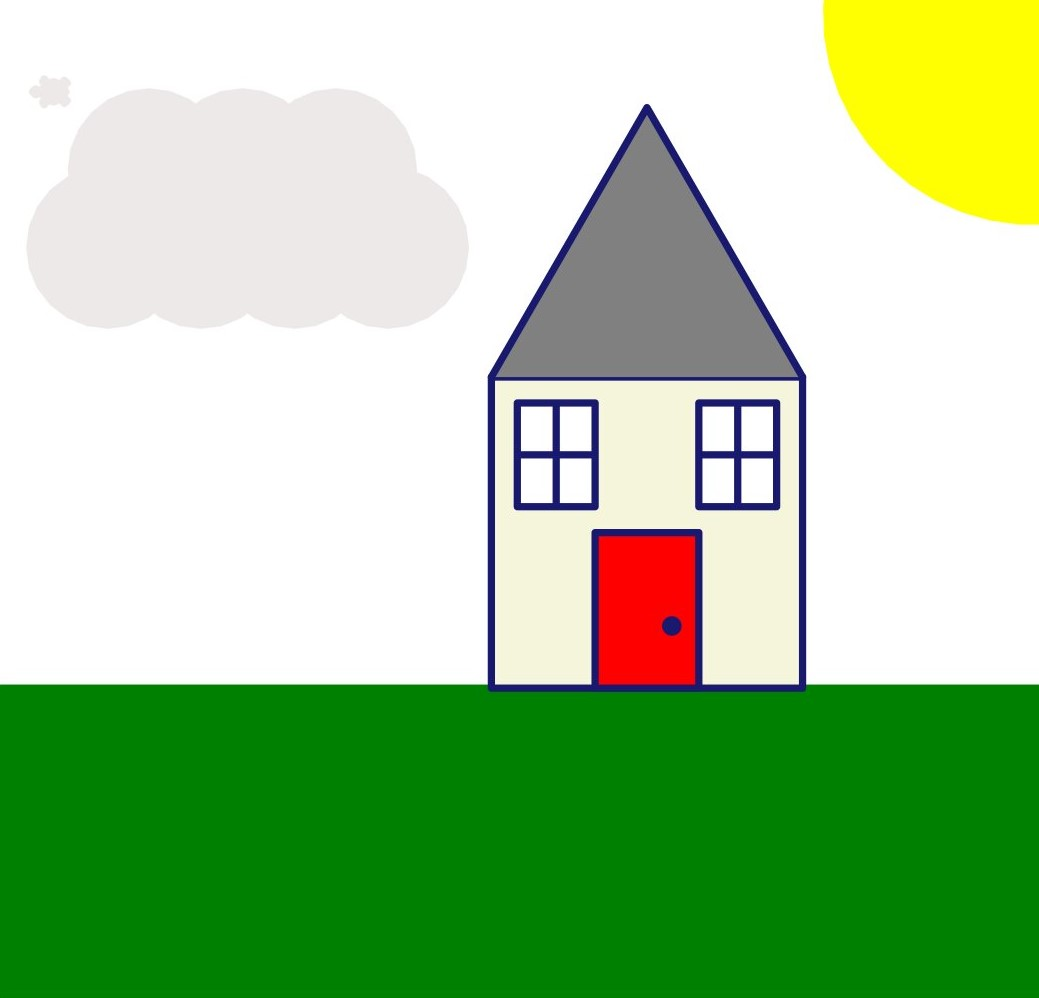
\includegraphics[scale=.2]{house_drawing}
\includegraphics[scale=.18]{drawing_example2}


\includegraphics[scale=.5]{turtle2.jpg}

\end{center}
    \section{How to submit.}

    Submit your project to Gradescope using the standard course submission procedures. 
    \newpage
    \section{Grading Rubric:}  \\
    \begin{enumerate}
        \item \textbf{Creativity}: Project produces a unique output that is visually appealing and displays some amount of planning and effort.
        \item \textbf{Diverse use of turtle methods}: Project employs more than just the basic turtle methods. Shows a deeper knowledge of how turtles work and how to manipulate them with more advanced and efficient code.
        \item \textbf{Use of for loops}: Project displays a basic understanding of for loops. Project uses at least one loop to generate at least one piece of their final image. Student must be able to explain how the loop contributed to the final image.
        \item \textbf{Interesting use of Python operators to generate designs}: Project uses one or more Python operators or functions that allows for a design that would have otherwise not been possible to make or at least would have incredibly difficult to achieve manually. 

        
    \end{enumerate}
    \section{Important Notes:} 
    \begin{enumerate}
        \item Note that the effective use of computer science concepts is worth more than the overall aesthetic of the final output. No matter how complicated the image is, it must reflect your coding abilities and grasp of key course concepts. We want to see you experiment and be creative with both your final image \emph{and} the code that you use to produce it. The amount of effort put into this project will be clear, and the project will be graded accordingly.
        \item You must be able to explain your code in a reasonable amount of detail to the grader that you will be meeting with. This will demonstrate to them that you understand the code that you have written. If you are unable to talk through your code, it is probably a sign that you need to visit TA hours or stop into your Professor's office hours for clarification. 
    \end{enumerate}


\end{document}
